% ==============================================================================
% sci_s4_pid.tex — SCI/SICE tutorial Session 4: feedback control basics, PID
% attitude stabilisation (14:00-15:00)
% SCI/SICE チュートリアル セッション4: フィードバック制御の基礎
% --- PID による姿勢安定化（14:00-15:00）
% ==============================================================================

% Fallback so this chapter still builds standalone (make chapter NAME=sci_s4_pid)
% before chapters/sci_intro.tex has run. In the full deck sci_intro defines the
% real \scisessionmap (five-session map, N highlighted) first, so this no-ops there.
% chapters/sci_intro.tex 読み込み前でも単体ビルドできるようにするフォールバック。
% フルビルドでは sci_intro が本物の \scisessionmap（5セッション地図、N強調）を
% 先に定義するため、ここでは何もしない。
\providecommand{\scisessionmap}[1]{}

% ------------------------------------------------------------------
\begin{frame}{地図: 今ここ}
  \begin{columns}[T]
    \begin{column}{0.5\textwidth}
      \centering
      \resizebox{\columnwidth}{!}{\scisessionmap{4}}
    \end{column}
    \begin{column}{0.47\textwidth}
      \small
      S2・S3 で組み上げた機体を、本セッションでは制御理論と突き合わせて飛ばす。
      「設計 $\to$ 実装」の次にくる「実験」のフェーズにあたる。

      \vspace{0.5em}

      \begin{block}{今日のセッションで扱うもの}
        \footnotesize
        レート P 制御の初飛行 $\to$ プラントモデルによる裏付け $\to$ PID 化 $\to$
        姿勢推定 $\to$ 実機データでの検証
      \end{block}
    \end{column}
  \end{columns}
\end{frame}

% ------------------------------------------------------------------
\begin{frame}{要点3つ}
  \begin{enumerate}
    \item モータ+機体のプラント伝達関数 $G_p(s) = K/(s(\tau_m s+1))$ を実測パラメータから導出し，ゲイン設計に使う
    \item P 制御から PID 化し，不完全微分・アンチワインドアップ・積分リセットまで含めたvehicle 実装と学習者コードを対比する
    \item フライトデータからプラントを同定し，設計値と実測値を突き合わせる
  \end{enumerate}

  \vspace{0.5em}

  \begin{alertblock}{本セッションの立ち位置}
    \small
    ここまでのレッスンは動かすことが目的だった。ここからは，動いた結果を
    モデルと数値で説明できるかを問う
  \end{alertblock}
\end{frame}

% ------------------------------------------------------------------
\begin{frame}{内側ループ: レート制御}
  \begin{center}
    \resizebox{0.85\textwidth}{!}{\documentclass[border=10pt]{standalone}
\usepackage{tikz}
\usetikzlibrary{arrows.meta, positioning, shapes.geometric, calc}

\begin{document}

\definecolor{blockcolor}{RGB}{0, 120, 200}
\definecolor{arrowcolor}{RGB}{80, 80, 80}
\definecolor{fbcolor}{RGB}{220, 50, 30}
\definecolor{sumcolor}{RGB}{40, 160, 40}
\begin{tikzpicture}[
    block/.style={
      rectangle, draw=blockcolor, line width=1.5pt,
      fill=blockcolor!8, rounded corners=3pt,
      minimum width=26mm, minimum height=14mm,
      font=\bfseries, text=blockcolor, align=center
    },
    % Summing-junction circle diameter is ~40% of block height (Block
    % Diagram Style convention), not 71% as before (10mm / 14mm block).
    % 加え合わせ点の円の直径はブロック高さの約4割（ブロック線図の流儀）。
    % 以前は 10mm / ブロック高さ14mm = 71% だった。
    sum/.style={
      circle, draw=sumcolor, line width=1.5pt,
      fill=sumcolor!8, minimum size=6mm,
      font=\normalsize\bfseries, text=sumcolor
    },
    arrow/.style={-{Stealth[length=3mm]}, line width=1.2pt, arrowcolor},
    lbl/.style={font=\small, above, text=arrowcolor},
  ]

  % Blocks
  \node[block] (target) at (0, 0) {Target\\Rate};
  \node[sum]   (sum)    at (3, 0) {$\Sigma$};
  \node[block] (kp)     at (6, 0) {P Control\\$K_p \times e$};
  \node[block] (mixer)  at (9.5, 0) {Motor\\Mixer};
  \node[block] (drone)  at (13, 0) {StampFly\\Drone};

  % Forward path
  \draw[arrow] (target) -- node[lbl] {$r$} (sum);
  \draw[arrow] (sum) -- node[lbl] {$e$} (kp);
  \draw[arrow] (kp) -- node[lbl] {$u$} (mixer);
  \draw[arrow] (mixer) -- (drone);

  % Output line with feedback tap point
  \draw[arrow] (drone.east) -- ++(2.5, 0) node[lbl, right] {response};
  \coordinate (fb_tap) at ($(drone.east)+(1.2, 0)$);
  \fill[arrowcolor] (fb_tap) circle (2.5pt);

  % Feedback path (branches from output line, not from inside drone)
  \node[block, fill=fbcolor!8, draw=fbcolor, text=fbcolor]
    (gyro) at (8, -3) {Gyro\\Sensor};
  \draw[arrow, fbcolor] (fb_tap) -- (fb_tap |- gyro) -- (gyro);
  \draw[arrow, fbcolor] (gyro) -- (3, -3) -- (sum);

  % Sum signs: "+" above the left-entering arrow, "-" to the RIGHT of the
  % bottom-entering feedback arrow (Block Diagram Style convention).
  % 加え合わせ点の符号: 「+」は左から入る矢印の上、「-」は下から入る
  % フィードバック矢印の右側に置く（ブロック線図の流儀）。
  % Fix: the "-" was at 210 deg (left of the upward arrow) with anchor
  % "north east" (glyph extending further left) -- it sat on the WRONG
  % (left) side of the arrow. Moved to 330 deg (right of the arrow) with
  % anchor "north west" (glyph extending right of the point).
  % 修正: 以前「-」は210度（上向き矢印の左側）・anchor=north east
  % （グリフがさらに左に伸びる）で、矢印の誤った（左）側にあった。
  % 330度（矢印の右側）・anchor=north west（グリフが右に伸びる）へ移動。
  \node[font=\scriptsize, sumcolor, anchor=south east] at ($(sum.north)+(150:0.3)$) {$+$};
  \node[font=\scriptsize, fbcolor, anchor=north west] at ($(sum.south)+(330:0.3)$) {$-$};

  % Labels
  \node[font=\small, arrowcolor, above] at ($(drone.east)+(1.2, 0.5)$) {angular rate};
  \node[font=\small, fbcolor, below] at (8, -3.8) {feedback};

\end{tikzpicture}
\end{document}
}
  \end{center}

  \vspace{0.5em}

  \begin{itemize}\small
    \item この図は\textbf{内側ループ（レート制御）}: 目標角速度とジャイロ計測値の差を制御。
          ACRO はこのループ単体で完結する
    \item \textbf{外側ループ（姿勢制御）}は，この図の入力 Target Rate を作る側にもう1段乗る。
          目標姿勢角と推定角の差から目標角速度を作り，STABILIZE 以上で有効になる
          （カスケード = ループの入れ子）
  \end{itemize}
\end{frame}

% ------------------------------------------------------------------
\begin{frame}{PID 制御器}
  \begin{center}
    \resizebox{0.78\textwidth}{!}{\documentclass[border=10pt]{standalone}
\usepackage{tikz}
\usepackage{amsmath}
\usetikzlibrary{arrows.meta, positioning, shapes.geometric, calc}

\begin{document}

\definecolor{pcolor}{RGB}{0, 120, 200}    % Blue - P
\definecolor{icolor}{RGB}{40, 160, 40}    % Green - I
\definecolor{dcolor}{RGB}{220, 50, 30}    % Red - D
\definecolor{arrowcolor}{RGB}{80, 80, 80}
\definecolor{sumcolor}{RGB}{120, 80, 150} % Purple - sum
\begin{tikzpicture}[
    block/.style={
      rectangle, draw=#1, line width=1.5pt,
      fill=#1!8, rounded corners=3pt,
      minimum width=38mm, minimum height=13mm,
      font=\bfseries, text=#1, align=center
    },
    % Summing-junction circle diameter is ~40% of block height (Block
    % Diagram Style convention), not 77% as before (10mm / 13mm block).
    % 加え合わせ点の円の直径はブロック高さの約4割（ブロック線図の流儀）。
    % 以前は 10mm / ブロック高さ13mm = 77% だった。
    sum/.style={
      circle, draw=sumcolor, line width=1.5pt,
      fill=sumcolor!8, minimum size=5.5mm,
      font=\normalsize\bfseries, text=sumcolor
    },
    arrow/.style={-{Stealth[length=3mm]}, line width=1.2pt, arrowcolor},
  ]

  % Input
  \node[font=\bfseries, arrowcolor] (input) at (-1, 0) {$e(t)$};

  % Branch point
  \coordinate (branch) at (1.5, 0);
  \fill[arrowcolor] (branch) circle (2.5pt);

  % P block (top)
  \node[block=pcolor] (P) at (5.5, 2) {P: $K_p \cdot e$};

  % I block (center)
  \node[block=icolor] (I) at (5.5, 0) {I: $\dfrac{K_p}{T_i} \displaystyle\int e\,dt$};

  % D block (bottom) -- Incomplete derivative filter
  \node[block=dcolor] (D) at (5.5, -2) {D: $K_p \cdot \dfrac{T_d s}{\eta T_d s + 1}$};

  % Sum
  \node[sum] (sum) at (10, 0) {$\Sigma$};

  % Output
  \node[font=\bfseries, arrowcolor] (output) at (12.5, 0) {$u(t)$};

  % Input arrow to branch
  \draw[arrow] (input) -- (branch);

  % Branch to P/I/D
  \draw[arrow, pcolor] (branch) |- (P);
  \draw[arrow, icolor] (branch) -- (I);
  \draw[arrow, dcolor] (branch) |- (D);

  % P/I/D to sum
  \draw[arrow, pcolor] (P) -| (sum);
  \draw[arrow, icolor] (I) -- (sum);
  \draw[arrow, dcolor] (D) -| (sum);

  % Sum to output
  \draw[arrow] (sum) -- (output);

  % Plus signs at sum.
  % Fix: the I-branch "+" was at 180 deg, exactly on the horizontal I-sum
  % arrow's own axis, so it was hidden under the arrowhead. Moved to
  % 160 deg (off-axis, slightly above) with a larger radius for clearance.
  % 修正: I分岐の「+」は180度（I→Sumの水平矢印の軸線上）にあり、矢頭の
  % 下に隠れていた。矢印の軸から外れる160度（軸よりやや上）へ移動し、
  % 半径も少し広げて余裕を持たせた。
  \node[font=\scriptsize, pcolor] at ($(sum)+(120:0.7)$) {$+$};
  \node[font=\scriptsize, icolor] at ($(sum)+(160:0.85)$) {$+$};
  \node[font=\scriptsize, dcolor] at ($(sum)+(240:0.7)$) {$+$};

  % Labels
  \node[font=\small, pcolor, anchor=south west] at (7.5, 2) {Proportional};
  \node[font=\small, icolor, anchor=south west] at (7.5, 0) {Integral};
  \node[font=\small, dcolor, anchor=north west] at (7.5, -2) {Incomplete Derivative};

  % Transfer function (below diagram)
  \node[font=\normalsize, arrowcolor, anchor=north] at (5.5, -3.8) {%
    $C(s) = K_p\!\left(1 + \dfrac{1}{T_i s} + \dfrac{T_d s}{\eta T_d s + 1}\right)$};

\end{tikzpicture}
\end{document}
}
  \end{center}
\end{frame}

% ------------------------------------------------------------------
\begin{frame}{プラントモデル}
  \begin{center}
    \vspace{-2mm}
    \resizebox{0.85\textwidth}{!}{\input{../../_shared/tikz/plant_model}}
  \end{center}

  \vspace{-0.5em}

  \begin{exampleblock}{ホバー近傍で線形化すると2ブロックに集約できる}
    \begin{itemize}
      \item \textbf{Mixer + Motor}: duty $\to$ トルク，1次遅れ $K_m/(\tau_m s+1)$
      \item \textbf{Body}: トルク $\to$ 角速度，積分器 $1/(I \cdot s)$
    \end{itemize}
  \end{exampleblock}
\end{frame}

% ------------------------------------------------------------------
\begin{frame}{実測パラメータ}
  \begin{table}
    \centering\small
    \begin{tabular}{llccc}
      \hline
      \textbf{パラメータ} & \textbf{記号} & \textbf{Roll} & \textbf{Pitch} & \textbf{Yaw} \\
      \hline
      慣性モーメント & $I$ & 9.16e-6 & 13.3e-6 & 20.4e-6\,kg$\cdot$m$^2$ \\
      トルクゲイン   & $K_m$ & 9.3e-4 & 9.3e-4 & 1.6e-4\,N$\cdot$m \\
      モータ時定数   & $\tau_m$ & \multicolumn{3}{c}{0.02\,s（共通，実測 0.0163\,s）} \\
      \hline
      \textbf{プラントゲイン} & $K = K_m/I$ & \textbf{102} & \textbf{70} & \textbf{8.0}\,rad/s$^2$ \\
      \hline
    \end{tabular}
  \end{table}

  {\tiny 注: この $K_m$（duty$\to$トルク，N$\cdot$m）はモータの逆起電力定数
  （back-EMF constant，V/(rad/s)，\code{docs/architecture/stampfly-parameters.md}）
  とは別物（記号が同じだけ）}

  \vspace{0.3em}

  \begin{exampleblock}{軸ごとに $K$ が違う理由}
    \footnotesize
    Roll/Pitch は同じ $K_m$ だが $I_{yy} > I_{xx}$ なので Pitch の方が遅い。
    Yaw は $\kappa \ll L$（トルク推力比がアーム長よりずっと小さい）ため
    $K_m$ 自体が小さく，さらに遅い
  \end{exampleblock}

  {\scriptsize 実習 6 配布コードの $K_{yaw}=19$（旧 $\kappa=9.71\times10^{-3}$\,m 由来）は
  この表の $K=8.0$（現行 $\kappa=4.10\times10^{-3}$\,m 由来）と異なる（後述の「PID 工学形式パラメータ」で詳述）}
\end{frame}

% ------------------------------------------------------------------
\begin{frame}{2次系設計}
  \vspace{-2mm}
  \begin{columns}[c]
    \begin{column}{0.38\textwidth}
      \centering
      \resizebox{\columnwidth}{!}{\input{../../_shared/tikz/step_response_zeta}}
    \end{column}
    \begin{column}{0.60\textwidth}
      \begin{block}{閉ループ伝達関数（2次系）}
        \setlength{\abovedisplayskip}{2pt}\setlength{\belowdisplayskip}{2pt}%
        \setlength{\abovedisplayshortskip}{2pt}\setlength{\belowdisplayshortskip}{2pt}%
        \[
          G_{cl}(s) = \frac{K_p K}{\tau_m s^2 + s + K_p K}
        \]
      \end{block}

      \vspace{0.2em}

      \begin{block}{$\zeta$ から $K_p$ を逆算する設計式}
        \setlength{\abovedisplayskip}{2pt}\setlength{\belowdisplayskip}{2pt}%
        \setlength{\abovedisplayshortskip}{2pt}\setlength{\belowdisplayshortskip}{2pt}%
        \[
          K_p = \frac{1}{4\zeta^2 K \tau_m}
        \]
      \end{block}

      \vspace{0.2em}

      {\small
      Roll/Pitch で $\zeta = 0.7$（オーバーシュート約5\%）を狙うと
      $K_{p,roll}=0.25$，$K_{p,pitch}=0.36$}
    \end{column}
  \end{columns}
\end{frame}

% ------------------------------------------------------------------
\begin{frame}{開ループボード線図}
  \begin{columns}[c]
    \begin{column}{0.50\textwidth}
      \centering
      \resizebox{\columnwidth}{!}{\input{../../_shared/tikz/bode_loop_shaping}}
    \end{column}
    \begin{column}{0.50\textwidth}
      \begin{block}{開ループ伝達関数}\small
        \setlength{\abovedisplayskip}{2pt}\setlength{\belowdisplayskip}{2pt}%
        \setlength{\abovedisplayshortskip}{2pt}\setlength{\belowdisplayshortskip}{2pt}%
        \[
          L(s) = K_p \cdot G_p(s) = \frac{K_p K}{s(\tau_m s + 1)}
        \]
      \end{block}

      \vspace{0.3em}

      {\small $K_p$ を上げるとゲイン交差周波数 $\omega_{gc}$ が上がり，位相余裕（PM）は下がる。
      P 制御だけでは応答速度と安定性がトレードオフの関係にある}
    \end{column}
  \end{columns}
\end{frame}

% ------------------------------------------------------------------
\begin{frame}{無駄時間の影響}
  \begin{columns}[c]
    \begin{column}{0.48\textwidth}
      \centering
      \resizebox{\columnwidth}{!}{\input{../../_shared/tikz/bode_dead_time}}
    \end{column}
    \begin{column}{0.52\textwidth}
      \begin{block}{制御ループの無駄時間}\small
        \setlength{\abovedisplayskip}{2pt}\setlength{\belowdisplayskip}{2pt}%
        \setlength{\abovedisplayshortskip}{2pt}\setlength{\belowdisplayshortskip}{2pt}%
        $\tau_d \approx 5$\,ms（センサ処理 + 制御演算 + PWM 更新）
        \[
          L_{delay}(s) = L(s)\cdot e^{-\tau_d s}
        \]
      \end{block}

      \vspace{0.3em}

      \begin{alertblock}{\small 実用上 PM $\geq 60°$ が必要}\scriptsize
        モデル上は安定なゲインでも，無駄時間を足すと実機で振動することがある
      \end{alertblock}
    \end{column}
  \end{columns}
\end{frame}

% ------------------------------------------------------------------
\begin{frame}[fragile]{実習 5 の振り返り: レート P 制御}
  \begin{sflisting}[basicstyle=\ttfamily\scriptsize]{user\_code.cpp（実習 5）}
float Kp_rp=0.5f, Kp_yaw=2.0f, rmax=1.0f, ymax=5.0f;
float re = ws::rc_roll()*rmax  - ws::gyro_x();
float pe = ws::rc_pitch()*rmax - ws::gyro_y();
float ye = ws::rc_yaw()*ymax   - ws::gyro_z();
ws::motor_mixer(ws::rc_throttle(),
    Kp_rp*re, Kp_rp*pe, Kp_yaw*ye);
  \end{sflisting}

  \vspace{0.5em}

  {\small 実習 5 では飛ばして安定するかどうかだけを見た。$K_p=0.5$ は勘で決めた値である}
\end{frame}

% ------------------------------------------------------------------
\begin{frame}{モデルで見る実習 5 の設計}
  \begin{table}
    \centering\small
    \begin{tabular}{lcc}
      \hline
      & \textbf{Roll（$K=102$）} & \textbf{Pitch（$K=70$）} \\
      \hline
      実習 5 の $K_p=0.5$ での $\zeta$ & 0.50 & 0.60 \\
      $\zeta=0.7$ 設計の $K_p$     & 0.25 & 0.36 \\
      \hline
    \end{tabular}
  \end{table}

  \vspace{0.5em}

  \begin{exampleblock}{読み取り}
    \footnotesize
    実習 5 の $K_p=0.5$ は Roll で $\zeta=0.50$，やや振動的な設定だったとモデルが説明する。
    P 制御だけでは，ゲインを下げて安定性を確保すると定常偏差と外乱への弱さが残る。
    ここから I 項・D 項を追加する
  \end{exampleblock}
\end{frame}

% ------------------------------------------------------------------
\begin{frame}{PID 工学形式パラメータ}
  \begin{table}
    \centering\scriptsize
    \renewcommand{\arraystretch}{0.95}
    \begin{tabular}{llp{58mm}}
      \hline
      \textbf{パラメータ} & \textbf{意味} & \textbf{効果} \\
      \hline
      $K_p$  & 比例ゲイン   & 大きいほど応答が速い，大きすぎると振動 \\
      $T_i$  & 積分時間 [s] & 小さいほど積分が強く効き偏差が早く消える \\
      $T_d$  & 微分時間 [s] & 大きいほど微分が強く効き振動を抑える \\
      $\eta$ & フィルタ係数  & $0.1\sim0.2$，大きいほどノイズに強い \\
      \hline
    \end{tabular}
  \end{table}

  \vspace{-0.35em}
  \begin{block}{教科書形式との対応（この形は vehicle の \code{rate.<axis>.kp/ti/td} が使う）}\footnotesize
    $K_i = K_p / T_i\,,\quad K_d = K_p \cdot T_d$（逆に $T_i = K_p/K_i,\ T_d = K_d/K_p$）
  \end{block}

  \vspace{-0.3em}
  {\scriptsize 実習 8 の解答は工学形式ではなく直接ゲイン $(K_p,K_i,K_d)$ を使う：
  Roll $(0.25,0.3,0.005)$，Pitch $(0.36,0.3,0.005)$，Yaw $(2.0,0.5,0.01)$
  （$K_p$ は Roll/Pitch が前ページの $\zeta=0.7$ 設計値，Yaw のみ経験値）。
  換算 $(T_i,T_d)$：Roll $(0.83\text{s},0.020\text{s})$，Pitch $(1.2\text{s},0.014\text{s})$，
  Yaw $(4.0\text{s},0.005\text{s})$。不完全微分フィルタと $\eta$ は未使用
  （vehicle 実装が追加する改良点）}
  \par
  {\scriptsize 実習 6 の配布コードは $\kappa$ 改定前の $K_{yaw}=19$（$K_p=1.34$）のまま。
  現行 $\kappa=4.10\times10^{-3}$\,m の $K=8.0$ を前ページの設計式に適用すると
  $K_p=3.19$ になり，設計式で追い直せる例として挙げる}
\end{frame}

% ------------------------------------------------------------------
\begin{frame}[fragile]{D 項とアンチワインドアップ}
  \begin{columns}[T]
    \begin{column}{0.5\textwidth}
      \begin{block}{実習 8 学習者コード}\scriptsize
        誤差の後退差分 D + 積分クランプ（フィルタ・条件分岐なし）
      \end{block}
      \begin{lstlisting}[style=sfcpp, basicstyle=\ttfamily\scriptsize]
// D term: raw backward difference
float D = Kd*(err-prev_err)/dt;

// Anti-windup: clamp the integral itself
integral += err*dt;
integral = clamp(integral, 0.5f);
float I = Ki*integral;
      \end{lstlisting}
    \end{column}
    \begin{column}{0.5\textwidth}
      \begin{alertblock}{vehicle 実装: sf\_controller\_pid}\scriptsize
        D項に不完全微分フィルタ（$\eta=0.125$）を追加し，誤差ではなく
        \textbf{測定値}に掛ける（D-on-M）。目標値が階段状に変わっても
        微分キックが出ない
      \end{alertblock}
      \begin{exampleblock}{アンチワインドアップ}\scriptsize
        単純な積分クランプではなく，出力が飽和方向に押される間だけ
        積分を止める「条件付き積分」を使う
      \end{exampleblock}
    \end{column}
  \end{columns}

  {\scriptsize 実習 8 の積分は $\pm0.5$ のクランプのみ（disarm 中は毎ループ 0 に戻る）。
  D-on-M・条件付き積分・不完全微分フィルタは vehicle 実装が追加する改良点
  （学習者コードへの拡張課題にもなる）。\code{sf\_controller\_pid/include/pid.hpp}
  が vehicle 実装のコード}
\end{frame}

% ------------------------------------------------------------------
\begin{frame}{離散化と ARM 時リセット}
  \begin{block}{離散化: 双一次変換（Tustin，vehicle 実装）}\small
    \code{sf\_controller\_pid} は比例・積分・微分に双一次変換を使う（$\alpha, a, b$ の式）。
    実習 8 は後退差分 D と矩形積分（Tustin ではない）
  \end{block}

  \vspace{0.3em}

  \begin{exampleblock}{積分リセットのタイミング（vehicle 実装）}\small
    積分器は DISARM 中ずっとゼロなのではなく，\textbf{ARM 遷移のたびに}
    リセットされる。着地して DISARM し，次に ARM した瞬間に積分が空になり，
    前のフライトの偏差を引きずらない
  \end{exampleblock}

  \vspace{0.3em}

  {\footnotesize
  ライブチューニング（\code{param set} での即時反映）では，積分器の状態は
  \textbf{保持}される。ゲイン変更のたびにループを蹴らないための区別。
  実習 8 は disarm 中は毎ループ 0 に戻り，結果として同じ効果になる}
\end{frame}

% ------------------------------------------------------------------
\begin{frame}{姿勢推定: ジャイロドリフト問題}
  \begin{columns}[c]
    \begin{column}{0.48\textwidth}
      \centering
      \resizebox{\linewidth}{!}{\input{../../_shared/tikz/gyro_drift}}
    \end{column}
    \begin{column}{0.50\textwidth}
      \begin{itemize}\small
        \item ジャイロは角速度 $\omega$ を測定，角度は積分 $\theta=\int\omega\,dt$ が必要
        \item バイアスが蓄積し，ドリフトが増大する
      \end{itemize}
      \vspace{0.5em}
      \begin{alertblock}{問題}\small
        ジャイロ単体では長時間の姿勢推定ができない。STABILIZE 以上で
        姿勢角を目標にするには，角度そのものの推定が要る
      \end{alertblock}
    \end{column}
  \end{columns}
\end{frame}

% ------------------------------------------------------------------
\begin{frame}{相補フィルタと STABILIZE}
  \begin{columns}[c]
    \begin{column}{0.50\textwidth}
      \centering
      \resizebox{\linewidth}{!}{\documentclass[border=10pt]{standalone}
\usepackage{tikz}
\usetikzlibrary{arrows.meta, positioning, calc}

\begin{document}

\definecolor{sfblue}{RGB}{0, 120, 200}
\definecolor{sfred}{RGB}{220, 50, 30}
\definecolor{sfgreen}{RGB}{40, 160, 40}
\definecolor{sfgray}{RGB}{80, 80, 80}
\definecolor{sflight}{RGB}{220, 240, 255}

\begin{tikzpicture}[
    node distance=1.5cm and 1.5cm,
    block/.style={draw, #1, line width=1.2pt, fill=#1!8,
                  minimum width=2.0cm, minimum height=0.9cm,
                  font=\normalsize\bfseries, rounded corners=3pt},
    block/.default=sfblue,
    gain/.style={draw, #1, line width=1.2pt, fill=#1!8,
                 circle, minimum size=0.9cm,
                 font=\normalsize\bfseries},
    gain/.default=sfblue,
    % Summing-junction circle diameter ~40% of block height (Block Diagram
    % Style convention; matches feedback_block.tex / pid_block.tex).
    % 加え合わせ点の円の直径はブロック高さの約4割（ブロック線図の流儀。
    % feedback_block.tex / pid_block.tex と揃える）。
    sum/.style={draw, sfblue, line width=1.2pt, fill=white,
                circle, minimum size=0.4cm,
                font=\normalsize\bfseries},
    input/.style={font=\normalsize\bfseries, sfgray},
    output/.style={font=\large\bfseries, sfblue},
    line/.style={-{Stealth[length=2.5mm]}, line width=1.2pt, sfgray},
    pathlbl/.style={font=\normalsize\bfseries},
  ]

  % --- Main path (gyro row): omega -> x(Delta t) -> Sigma1 -> alpha -> Sigma2 -> output ---
  % 主経路（ジャイロ行）: ω → ×Δt → Σ1 → α → Σ2 → 出力
  \node[input] (gyro_in) {Gyro $\omega$};
  \node[block=sfred, right=1.3cm of gyro_in] (dt_block) {$\times\Delta t$};
  \node[sum, right=1.3cm of dt_block] (sum1) {$\Sigma$};
  \node[gain=sfred, right=1.3cm of sum1] (alpha) {$\alpha$};
  \node[sum, right=1.3cm of alpha] (sum2) {$\Sigma$};
  \node[output, right=1.1cm of sum2] (output) {$\hat{\theta}$};

  % --- Accel path (top row): drops into Sigma2 from above, entirely outside
  %     the gyro feedback loop below (which stays self-contained around
  %     Sigma1). This is the layout fix versus the previous revision, where
  %     the accel row sat below the main row and visually nested inside the
  %     feedback loop even though it carries no feedback signal. ---
  % 加速度経路（上段）: Σ2 に上から入る。下側のジャイロ・フィードバック
  % ループ（Σ1周りで閉じる）とは完全に別の場所を通る。旧版は加速度経路が
  % 主経路の下段にあり，フィードバック信号ではないのに見た目上ループの
  % 内側に入り込んでいた。これを是正したのが今回のレイアウト。
  \node[input, above=2.0cm of gyro_in] (accel_in) {Accel};
  \node[block=sfgreen, right=1.3cm of accel_in] (atan) {atan2};
  \node[gain=sfgreen, right=1.3cm of atan] (one_alpha) {$1\!-\!\alpha$};

  % --- Feedback delay path (below row): previous estimate theta_hat_{k-1} ---
  % フィードバック遅延経路（下段）: 前回推定値 θ̂_{k-1} を戻す
  \node[block=sfblue, below=1.5cm of sum1, minimum width=1.6cm] (delay) {$z^{-1}$};

  % --- Branch point on the output line (theta_hat is tapped, not re-derived) ---
  % 出力線上の分岐点（θ̂ をそのまま分岐、再計算しない）
  \coordinate (tap) at ($(sum2)!0.5!(output)$);

  % --- Connections: gyro path ---
  \draw[line, sfred] (gyro_in) -- (dt_block);
  \draw[line, sfred] (dt_block) -- (sum1.west);
  \draw[line, sfred] (sum1.east) -- (alpha.west);
  \draw[line, sfred] (alpha.east) -- (sum2.west);

  % --- Connections: accel path. Drops straight down into Sigma2 from the
  %     north; a short right-angle jog (down, then across) absorbs the
  %     small misalignment between one_alpha's x-position and sum2's,
  %     since "right=1.3cm of" spacing is computed from each row's own
  %     node widths and the two rows use different-width nodes. ---
  % 加速度経路の接続。Σ2 に北側からまっすぐ下りる。one_alpha と sum2 の
  % x座標のわずかなズレ（"right=1.3cm of" の間隔は各行のノード幅から
  % 計算されるため，幅の違う行同士では厳密には揃わない）を、
  % 短い直角ジョグ（下りてから横に寄せる）で吸収する。
  \draw[line, sfgreen] (accel_in) -- (atan);
  \draw[line, sfgreen] (atan) -- (one_alpha);
  \draw[line, sfgreen] (one_alpha.south) -- ++(0,-0.4) -| (sum2.north);

  % --- Output line and its branch dot ---
  \draw[line, sfblue, line width=1.5pt] (sum2) -- (output);
  \fill[sfblue] (tap) circle (2.2pt);

  % --- Feedback path: branch dot -> straight down -> into delay from the
  %     east -> up into Sigma1 from below. With the accel path now routed
  %     above the main row, the lower half-plane belongs to this path
  %     alone, so (unlike the previous revision) no detour around another
  %     signal is needed. ---
  % フィードバック経路: 分岐点 → まっすぐ下へ → 遅延ブロックへ東側から
  % 入る → 上へ → Σ1 に南側から入る。加速度経路が上段に移ったことで
  % 下半分はこの経路専用になり，旧版で必要だった他信号を避ける迂回が
  % 不要になった。
  \draw[line, sfblue] (tap) -- (tap |- delay.east) -- (delay.east);
  \draw[line, sfblue] (delay.north) -- (sum1.south);

  % --- Sum node signs (Block Diagram Style convention): "+" sits above a
  %     horizontally (west-)entering arrow. For a vertically-entering arrow
  %     (into Sigma1 from below, into Sigma2 from above) the "+" sits to
  %     the arrow's right, mirroring Sigma1's existing bottom-entry sign. ---
  % 加え合わせ点の符号（ブロック線図の流儀）: 水平（西側）から入る矢印の
  % 「＋」はその上に置く。垂直に入る矢印（Σ1は下から，Σ2は上から）の
  % 「＋」はその右側に置く（Σ1の下からの入力の符号と同じ規則）。
  \node[font=\scriptsize, sfred,  anchor=south east] at ($(sum1.north)+(150:0.3)$) {$+$};
  \node[font=\scriptsize, sfblue, anchor=north west] at ($(sum1.south)+(330:0.3)$) {$+$};
  \node[font=\scriptsize, sfred,  anchor=south east] at ($(sum2.north)+(150:0.3)$) {$+$};
  \node[font=\scriptsize, sfgreen, anchor=south west] at ($(sum2.north)+(30:0.3)$) {$+$};

  % --- Path labels (kept off the signal lines) ---
  \node[pathlbl, sfred, below=0.2cm of dt_block] {High-pass};
  \node[pathlbl, sfgreen, above=0.2cm of atan] {Low-pass};
  \node[pathlbl, sfblue, below=0.15cm of delay] {前回値};

\end{tikzpicture}
\end{document}
}
    \end{column}
    \begin{column}{0.48\textwidth}
      \begin{block}{数式}\footnotesize
        $\hat\theta_k = \alpha(\hat\theta_{k-1}+\omega\Delta t) + (1-\alpha)\theta_{accel}$
      \end{block}
      \vspace{0.3em}
      \begin{itemize}\small
        \item $\alpha=0.98$（ジャイロ98\% + 加速度2\%）
        \item StampFly の既定は 15 状態 ESKF。相補フィルタは自作して
              \api{estimated\_roll()} と比較する教材
      \end{itemize}
    \end{column}
  \end{columns}

  \vspace{0.3em}

  {\small STABILIZE ではこの推定角を外側ループの入力にし，スティックが
  傾き角そのものを指令する}
\end{frame}

% ------------------------------------------------------------------
\begin{frame}[fragile]{システム同定: sf sysid fit}
  \begin{block}{$K_p$ が既知なら，閉ループデータから開ループプラントを復元できる}
    \footnotesize $u(t) = K_p(\text{target}-\text{gyro})$，$y(t)=\text{gyro}$ として
    $G_p(s)=K/(s(\tau_m s+1))$ に最小二乗フィット
  \end{block}

  \vspace{0.5em}

  \begin{sflisting}[basicstyle=\ttfamily\scriptsize]{出力例}
sf sysid fit flight.csv --kp 0.5 --plot
  Roll  K= 98.5 (ref:102.0, err:3.4%) tau_m=0.019 R2=0.94
  Pitch K= 72.1 (ref: 70.0, err:3.0%) tau_m=0.021 R2=0.91
  \end{sflisting}

  {\small 理論値（実習 6）との誤差3〜4\%は，モデル簡略化と無駄時間の影響で説明できる}
\end{frame}

% ------------------------------------------------------------------
\begin{frame}[fragile]{自動チューニング: sf sysid rate-fit / rate-tune}
  \begin{block}{ETFE によるプラント同定と仕様ベースのゲイン設計}\footnotesize
    チャープ（またはダブレット）励振で軸ごとに $(b, L, T)$ を推定し，
    $G_p(s) = b\,e^{-Ls}/(s(Ts+1))$ にフィットする。sf sysid fit は P 制御のみ仮定の
    逆算だが，ここでは実際に飛んだ PID 出力（I・D 項含む）を再構成してから
    ETFE を取る閉ループ同定
  \end{block}

  \begin{sflisting}[basicstyle=\ttfamily\scriptsize]{コマンド}
sf sysid rate-fit flight.csv --axis roll -o fit.json
sf sysid rate-tune --fit fit.json --wc 25 --pm 60
  \end{sflisting}

  \vspace{-0.3em}
  {\footnotesize \code{rate-tune} はゲイン交差周波数 $\omega_c$ と位相余裕 PM の仕様を満たす
  $K_p/T_i/T_d$ を逆算し，\code{param set rate.roll.kp ...} の形で出力する}

  \vspace{-0.3em}
  {\scriptsize \warn{注:} 学習者コードで rate-fit/rate-tune を使うには，角速度目標を計算した
  直後に \api{ws::set\_rate\_target(roll,pitch,yaw)} を呼ぶ（実習 5 の解答でヒント導入・
  実習 7 で必須，Data Stream の \code{rate\_ref\_*} に記録される）}
\end{frame}

% ------------------------------------------------------------------
\begin{frame}{デモ: 完成コードで飛行}
  \begin{exampleblock}{デモの見方}\footnotesize
    \textbf{見るだけ}: ステップ応答の波形と設計値の一致を確認するだけで要点はつかめる。
    \textbf{一緒に打つ}: 手元の flight.csv で \code{sf sysid fit} を試す。
    \textbf{帰宅後に再現}: 本日は見るだけにして，後日実習 5〜9を通しで動かす
  \end{exampleblock}

  \begin{block}{手順}\footnotesize
    \begin{enumerate}
      \item PID 化した学習者コードで飛行し，\code{sf log wifi} でテレメトリ取得
      \item \code{sf log viz} でロール角速度のステップ応答を表示
      \item モデル予測（$\zeta=0.7$ の応答波形）と重ねて比較
    \end{enumerate}
  \end{block}
\end{frame}

% ------------------------------------------------------------------
\begin{frame}{デモの期待結果: P と PID のステップ応答}
  \begin{center}
    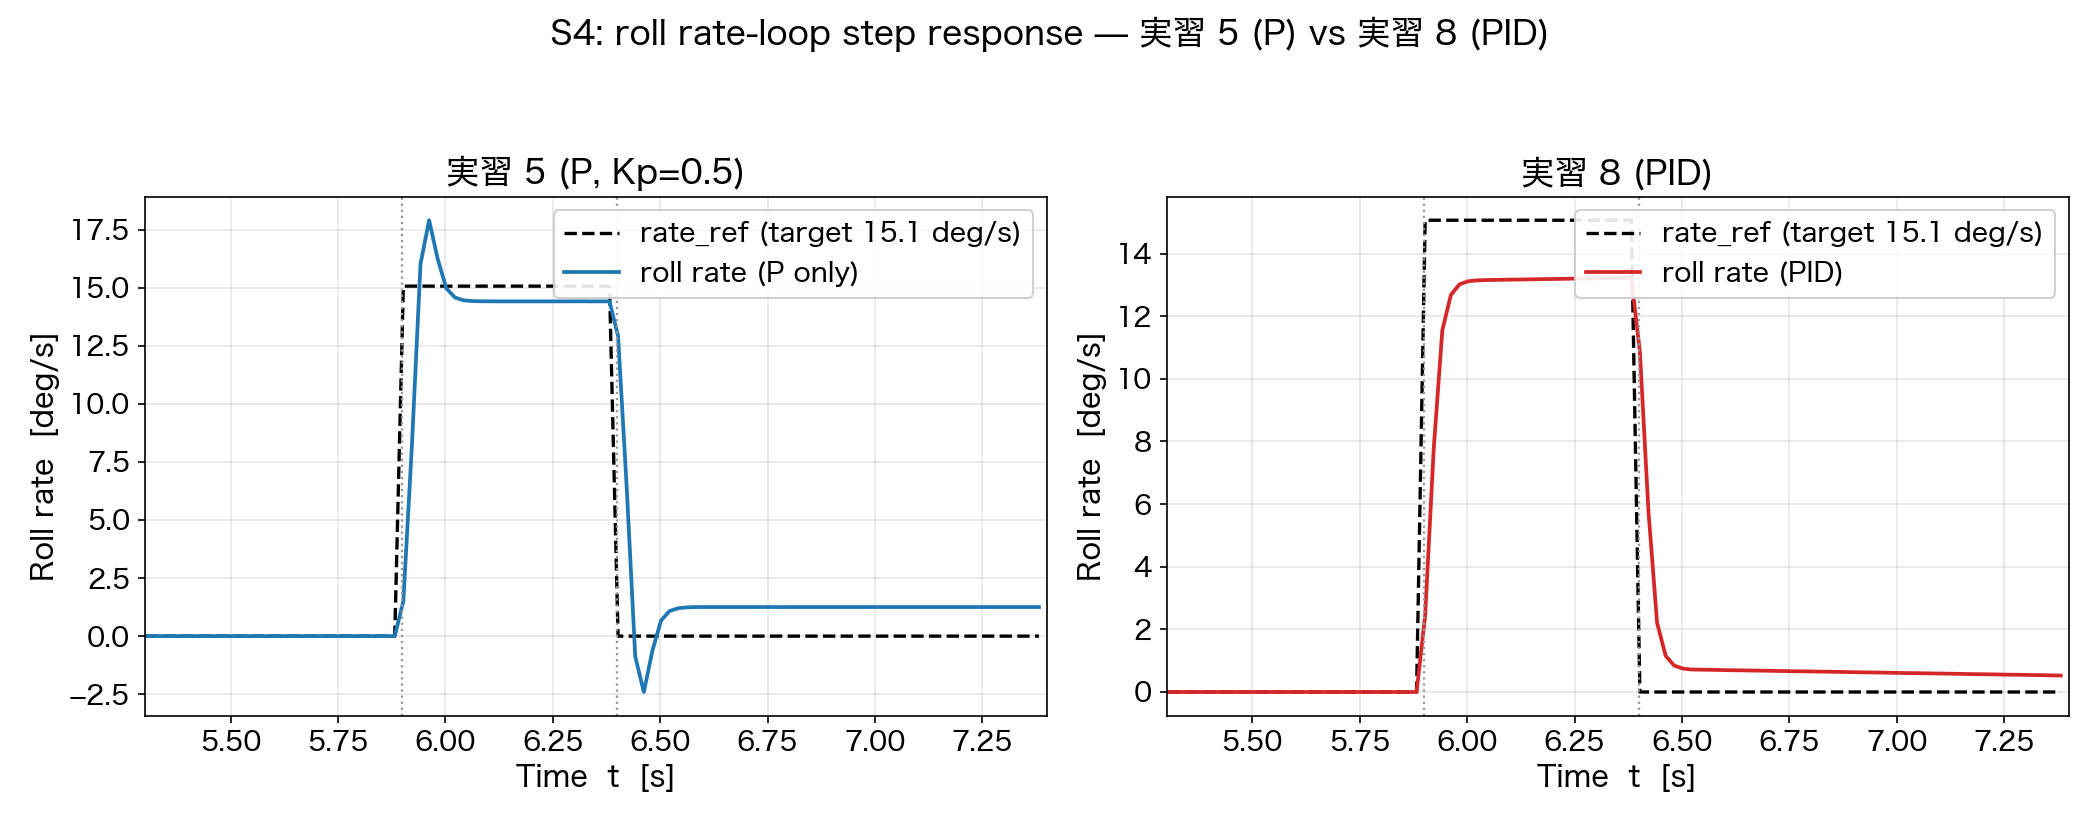
\includegraphics[width=\textwidth, height=0.46\textheight, keepaspectratio]{../fallback/S4_roll_step_p_vs_pid.png}
  \end{center}

  \vspace{0.2em}

  {\footnotesize SILS（MuJoCo）で \code{workshop\_acro\_step.scn}（ロール $+0.3$ を $0.5$\,s）を実行。
  目標 15.1\,deg/s に対し実習 5（P）はピーク 17.9\,deg/s と $-2.4$\,deg/s のアンダーシュート，
  実習 8（PID）はピーク 13.2\,deg/s で振動なし。角速度は真値ロール角の数値微分}
\end{frame}

% ------------------------------------------------------------------
\begin{frame}{発展の予告}
  \begin{itemize}\small
    \item \textbf{オートチューン}: \code{sf sysid rate-tune} と同じ $\omega_c$・PM 仕様のゲイン設計を
          機体上で行う \api{sf\_autotune}。励振はステップドサインで，周波数点ごとの I/Q 積算から
          $G(j\omega)$ を測り，プラントフィットまでオンボードで完結させる
    \item \textbf{ESKF}: 相補フィルタで自作した推定と，機体が実際に使う15状態
          ESKF の違い
    \item \textbf{高度・位置ループ}: 今日のレート/姿勢カスケードのさらに外側に
          高度・位置ループが乗る。S5 のシミュレータ活用で扱う
  \end{itemize}
\end{frame}

% ------------------------------------------------------------------
\begin{frame}{理論とコードの対応表}
  \resizebox{\textwidth}{!}{%
  \begin{tabular}{llll}
    \hline
    \textbf{教科書表記} & \textbf{実習 8 学習者コード} & \textbf{vehicle 実装} & \textbf{Data Stream} \\
    \hline
    比例ゲイン $K_p$   & \code{float Kp}（無次元） & \code{rate.roll.kp}（Nm/(rad/s)） & --- \\
    積分ゲイン $K_i$（$T_i{=}K_p/K_i$） & \code{float Ki}（直接ゲイン） & \code{rate.roll.ti}（s，換算値） & --- \\
    微分ゲイン $K_d$（$T_d{=}K_d/K_p$） & \code{float Kd}（フィルタなし） & \code{rate.roll.td}，$\eta$固定（実習8は未使用） & --- \\
    姿勢ゲイン          & ---（実習 8では未使用）    & \code{attitude.roll.kp/ti/td}      & --- \\
    目標角速度          & \code{target}             & \code{rate\_sp\_roll}              & \code{rate\_ref\_roll} \\
    角速度計測値        & \code{ws::gyro\_x()}      & \code{state.angular\_rate[0]}       & \code{gyro\_x} \\
    アンチワインドアップ & 積分クランプ $\pm0.5$     & 条件付き積分（\code{pid.hpp}）      & --- \\
    ARM 時リセット      & disarm 中毎ループ 0 に    & \code{PidController::reset()}（ARM遷移時） & --- \\
    \hline
  \end{tabular}}

  \vspace{0.5em}

  {\small レートループの $K_p$ は，学習者コードでは duty 空間の無次元値，
  vehicle 実装では物理トルク単位（ミキサーが推力配分に変換する前の値）。
  数値を単純比較できない点が「学習者コードと vehicle 実装の違い」を最もよく表す}
\end{frame}

% ------------------------------------------------------------------
\begin{frame}{復習パス}
  \resizebox{\textwidth}{!}{%
  \begin{tabular}{lll}
    \hline
    \textbf{コマンド} & \textbf{実習} & \textbf{文書} \\
    \hline
    \code{sf lesson switch sci2026:5} & 実習 5 レート P 制御 & Workshop Lesson 5 \\
    \code{sf lesson switch sci2026:6} & 実習 6 システムモデリング & Workshop Lesson 6 \\
    \code{sf sysid fit}               & 実習 7 システム同定 & Workshop Lesson 7 \\
    \code{sf lesson switch sci2026:8} & 実習 8 PID 制御      & Workshop Lesson 8 \\
    \code{sf lesson switch sci2026:9} & 実習 9 姿勢推定      & Workshop Lesson 9 \\
    \hline
  \end{tabular}}

  \vspace{0.5em}

  {\small すべて \code{sf lesson build} $\to$ \code{sf lesson flash} で実機に反映する。
  \code{--solution} で模範解答に切り替えられる}

  {\scriptsize Workshop スライド（\code{docs/events/stampfly\_workshop/slides/chapters/}）内の該当 Lesson 章に対応}
\end{frame}

% ------------------------------------------------------------------
\begin{frame}{チェックポイント}
  \begin{alertblock}{確認事項}
    \begin{itemize}
      \item[$\square$] $G_p(s)=K/(s(\tau_m s+1))$ と実測パラメータの対応を説明できる
      \item[$\square$] P 制御の限界と，I 項・D 項が何を補うかを説明できる
      \item[$\square$] 不完全微分・アンチワインドアップ・ARM 時リセットで
            学習者コードと vehicle 実装がどう違うか説明できる
      \item[$\square$] \code{sf sysid fit} の入出力と，理論値との比較の読み方を理解した
    \end{itemize}
  \end{alertblock}

  \vspace{1em}

  \begin{block}{次のセッション}
    S5: シミュレータ・解析ツールの活用と発展的テーマ（15:30 -- 16:30）
  \end{block}
\end{frame}
